\documentclass[10pt,twocolumn,hidelinks,letterpaper]{article}

\usepackage[table]{xcolor}
\usepackage{cvpr}
\usepackage{times}
\usepackage{epsfig}
\usepackage{graphicx}
\usepackage{amsmath}
\usepackage{amssymb}

\usepackage[utf8x]{inputenc}
\usepackage[english]{babel}
\usepackage{url}
\usepackage{lipsum}

\usepackage[framed, numbered]{matlab-prettifier}
\usepackage{listings}
\usepackage{setspace}
\usepackage{color} %red, green, blue, yellow, cyan, magenta, black, white
\usepackage{geometry}
\usepackage{subcaption}
\usepackage{graphicx}
\usepackage{float}


% Include other packages here, before hyperref.

% If you comment hyperref and then uncomment it, you should delete
% egpaper.aux before re-running latex.  (Or just hit 'q' on the first latex
% run, let it finish, and you should be clear).
\usepackage[breaklinks=true,bookmarks=false]{hyperref}

\cvprfinalcopy % *** Uncomment this line for the final submission

\def\cvprPaperID{****} % *** Enter the CVPR Paper ID here
\def\httilde{\mbox{\tt\raisebox{-.5ex}{\symbol{126}}}}

% Pages are numbered in submission mode, and unnumbered in camera-ready
%\ifcvprfinal\pagestyle{empty}\fi

\setcounter{page}{1}
\begin{document}

%%%%%%%%% TITLE
\title{01TXFSM - Machine Learning and Deep Learning \\
\vspace{0.3in}
Final Project \\
First Person Action Recognition}

\author{
  Eros Fanì - s269781\\
  Politecnico di Torino\\
  {\tt\small eros.fani@studenti.polito.it}
  \and
  Gabriele Trivigno - s276807\\
  Politecnico di Torino\\
  {\tt\small gabriele.trivigno@studenti.polito.it}
  \and
  Cristiano Gerbino - s277058\\
  Politecnico di Torino\\
  {\tt\small s277058@studenti.polito.it}
}

\maketitle
%\thispagestyle{empty}

\lstset{language=python,%
  %basicstyle=\color{red},
  breaklines=true,%
  morekeywords={matlab2tikz},
  keywordstyle={\small \color{blue}},%
  morekeywords=[2]{1}, keywordstyle=[2]{\small \color{black}},
  identifierstyle={\small \color{black}},%
  stringstyle={\small \color{mylilas}},
  commentstyle={\small \color{mygreen}},%
  showstringspaces=false,%without this there will be a symbol in the places where there is a space
  numbers=left,%
  numberstyle={\small \color{black}},% size of the numbers
  numbersep=7pt, % this defines how far the numbers are from the text
  emph=[1]{error,warning},emphstyle=[1]{\small \color{red}} %some words to emphasise
  %emph=[2]{word1,word2}, emphstyle=[2]{style},
}

%%%%%%%%% BODY TEXT
\newcommand{\quotes}[1]{“#1”}
\newcommand{\reff}[1]{Figure \ref{#1}}
\setlength{\parindent}{0pt}
\setstretch{0.1}
\setlength{\parskip}{1em}
\definecolor{TopRow}{HTML}{E6E6FF}

\begin{abstract}

The First Person Action Recognition problem is a trendy challenge of our times: due to the increasing popularity of wearable cameras, the interest on this field is more and more increasing among the researches. This is a really difficult task, starting from the problem of how to cope with the motion of the camera of the user, the amount of information that are available for the gatherering with a so strict focusing of the frames of the video, and often the lack of audio information. In our work we have dealt with egocentric mute videos: we have tried to classify fine-grained culinary actions by exploring the solutions proposed by other researches. After this preliminary work we put in practice some useful upgrades to these solutions, trying to merge them also with other approaches originally thought for other video recognition contexts.

\end{abstract}

\section{Introduction}
The main scope of this project was the field of First Person Action Recognition, which is one of the up-and-coming domains in modern Computer Vision, due to the recent spread of wearable devices, often camera-equipped.
Even though action recognition and video analysis in general have been topics of research for quite some time now, this particular task introduces some newly faced challenges such as the strong egomotion component, which is inevitable as cameras are placed directly on the actor. Moreover the First Person point of view lacks some important information about the actor and its pose, showing only a part of the scenario, making inference harder. The most frequently adopted techniques to tackle this issues combine spatial information, taken from RGB frames, and motion clues, extracted in various ways, such as temporal stream networks based on optical flow, attention modules or 3D CNNs. We will discuss in depth some of this methodologies, highlighting in our opinion what are the weaknesses of such approaches, and proposing possible ways to circumvent them.

\subsection{Goals}
The first goal of the project was to replicate the main results of \cite{egornn}. Afterwards, we integrated the cited architecture with the self-supervised block proposed in \cite{sparnet}, implementing it in 2 different ways.

After trying to replicate these experiments with the hyperparameters setting reported in \cite{egornn}, with the experience acquired we chose other sets of hyperparameters that could potentially fit better our dataset of interest, and so performed a grid search upon them.

At last we have tried to improve the performances of the results of \cite{egornn} and \cite{sparnet} with some innovative ideas of our own.


\subsection{Our contribution}

\section{Related works}
Existing literature has underlined how the must crucial information to encode into features in order to obtain good performances on the task of First Person Action Recognition are the hands motion of the actor, and the appearance of objects manipulated, as well as their interaction. Putting together this 2 fundamental pieces of information is perhaps the most challenging task, and more importantly doing so without complicating too much the architecture, which could lead to high computational costs, cutting of potential on-line applications. \cite{egornn} proposes a spatial attention mechanism to focus on the region consisting of the object, arguing that objects handled are strongly representative of egocentric activities. To keep track of said objects throughout frames, this spatial attention is paired with a with a convLSTM module, whose purpose is to temporal encode the frame-level features formerly extracted. In addition to this, they also use a temporal network fed with optical flow images, following the purpose of better encoding motion changes in the considered videos. The task is then addressed with a late fusion of the 2 outputs with a dense layer to finally perform the classification step. Whilst reasonably successful, this approach consists of a two stream network, which requires several training stages
resulting in a massive number of parameters to train. \cite{sparnet} argues that adding a self-supervised block which leverages motion maps at the output of the CNN backbone can provide the convLSTM module with a richer input that already encloses motion information. They show that in this way the network is able to obtain a meaningful enough representation of both appearance and movement to achieve state-of-the-art results, so that the temporal network is no longer needed. Many other works recognize the importance of slimming the architecture to avoid having to train a 2 stream network. \cite{motfilt} introduces a unified model that aims at representing spatio-temporal relationship using only RGB frames, eliminating the heavy computation time required to extract optical flow, which makes the most difference at test time, once the model has been deployed. In their MFNet they insert motion filter blocks in the middle of CNN layers, that act upon feature maps extracted from shared-networks feed-forwarded by two consecutive input frames. The flow is estimated moving each channel of these feature maps in a
different spatial direction $\delta := (\Delta x, \Delta y)$. \cite{reprflow}
argues that the procedure described, though advantageous parameter-wise and computation-wise, suffer from inferior performance compared with more powerful two-stream networks. They maintain such performance gap is due to the iterative optimization that standard optical flow methods implement and that \cite{motfilt} failes to reproduce. To overcome this issue they propose a new, fully-differentiable, layer, built to extract flow from any CNN feature map. By learning the flow parameters of a smaller resolution CNN tensor, in an end-to-end fashion together with the CNN training, they claim to
achieve the same representational power as traditional flow methods, and even better since flows optimized for activity recognition is different from true optical flow.
This last two works introduce a great way to encode motion clues in the features extracted, but none of them combine this information with a temporal representation of those features. Whereas \cite{egornn} fails to exploit RGB frames to get motion informations beyond appearances. Even though \cite{sparnet} tries to overcome this with the motion segmentation task, we found that their approach can sometimes lacks of precision in identifying the region of interest, since it acts on very high-level features.
In this project we propose three new different approaches. First of all, we use an improved version of the self-supervised block adopted in \cite{sparnet}to integrate in the work of \cite{egornn}, eliminating the need of a second network and improving the granularity of the motion encoding using higher resolution maps matched with lower level features. Afterwards we adopt the representation-flow layer proposed by \cite{reprflow} together with a temporal encoding module to better exploit temporal relationships in the features extracted. Finally we experimented with a different approach: encoding the concept of dynamics directly into the convLSTM module, adding a discriminator classifier that has been trained to discern whether it has been fed with static frames, or actual video frames.

\section{Methodologies overview}
Here we describe the models that we have used to perform our experiments.

\subsection{Egornn}
\textit{Egornn} is a CNN-RNN joint architecture presented in \cite{egornn}. The overall architecture of \textit{Egornn} is shown in \reff{egornn_arch}. The CNN backbone is based on \textit{resnet34}\cite{resnet}, which has five main building blocks: with respect to \reff{egornn_arch} they are: \textit{Conv}, \textit{Layer1}, \textit{Layer2}, \textit{Layer3} and , \textit{Layer4}. From now on we will refer to these blocks respectively \textit{conv1}, \textit{conv2}, \textit{conv3}, \textit{conv4} and \textit{conv5}. It is pree-trained for generic image recognition and complemented with an attention mechanism for spatially selective feature extractin that we are now going to describe.

The exit of \textit{conv5} is used to generate a \textit{Class Activation Map} (CAM). Let $f_l(i)$ be the activation of a unit l in the final convolutional layer
at spatial location i and $w_c^l$ be the weight corresponding to class c for unit l. Then the CAM
for class c, $M_c(i)$, can be represented as
\begin{equation*}
M_c(i) = \sum_{l} w_l^c f_l(i)
\end{equation*}
Computing this using only the winning class results in a saliency map of the image highlighting the region in which this object is contained. They argue that this is enough to focus on the object handled by the observer, but we are going to show that this is not always the case. Finally the CAM is converted to a probability spatial map using  softmax along the pixel, and multiplied again with the \textit{conv5} output to get the final spatial attention maps.
\begin{equation*}
f_{SA}(i) = f(i) \odot \frac{e^{M_c(i)} }{ \sum_{i^{'}} e^{M_c(i^{'})}}
\end{equation*}
where $f(i)$ represents the output feature from the final convolutional layer of ResNet-34 at
a spatial location i, $M_c(i)$ is the CAM obtained using the winning class c,
$f_{SA}(i)$ is the image feature after spatial attention is applied and $\odot$ represents the Hadamard product.

Afterwards the spatial attention is used to feed e convLSTM module that aims at getting a spatial-temporal encoding of the frame-level features extracted by the CNN backbone. It takes into account, for each frame $i$, both the output of the SAM for the layer i and the output of the ConvLSTM for the layer $i-1$, constituting a recurrent structure
This allows the network to learn relationship between spacial and temporal changes, though we argue that what this approach really does is memorize the appearance of an object throughout time, lacking the motion information, and we wll discuss more about this later. ConvLSTM is a RNN, and the difference with the standard LSTM is that it allows to track the spatial features thanks to its memory tensor, instead of the standard vectorial state. So all the multiplication with input, forget and output gates become convolutions. For each cell the equations are the following :
\begin{align*}
i_t = \sigma(w_x^i * f_{SA} + w_h^i * h_{t-1} + b^i)\\
f_t = \sigma(w_x^f * f_{SA} + w_h^f * h_{t-1} + b^f)\\
\tilde{c_t} = tanh(w_x^{\tilde{c}}*f_{SA}+w_h^{\tilde{c}}*h_{t-1} + b^{\tilde{c}})\\
c_t = \tilde{c_t} \odot f_{SA} + c_{t-1} \odot f_{t}\\
o_t = \sigma(w_x^o * f_{SA} + w_h^o * h_{t-1} + b^0)\\
h_t = o_t \odot tanh(c_t)
\end{align*}
where $\sigma$ is the sigmoid function, $i_t$, $f_t$, $o_t$, $c_t$ and $h_t$ represent the input state, forget state,
output state, memory state and hidden state, respectively, of the convLSTM. The trainable
weights and biases of the convLSTM are represented using w and b


The last output of the ConvLSTM (the output obtained from the last frame of a particular video) is average pooled and reshaped to obtain a final classification layer with 61 neurons (i.e. the number of classes of our dataset).

\begin{figure*}
  \centering
  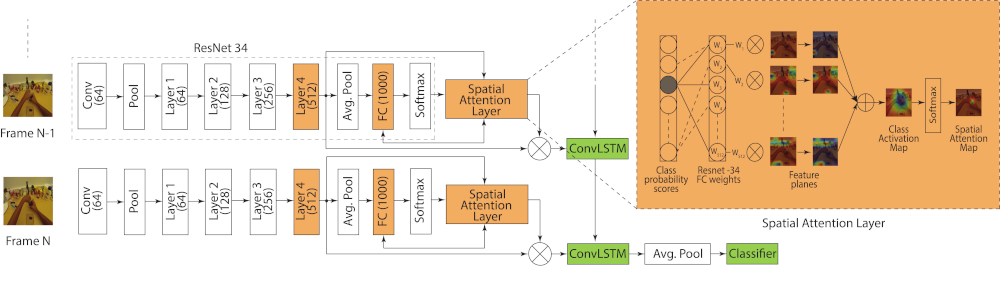
\includegraphics[width=\linewidth]{images/egornn.png}
  \caption{Architecture of \textit{egornn}}
  \label{egornn_arch}
\end{figure*}

\subsection{Flow\_resnet34}

\textit{Flow\_resnet34} is the second network used by \cite{egornn}. It is mainly just a \textit{resnet34}, trained separately to work with warp flows. As
warp flow are supposed to contain motion clues tied to spatial location, the purpose of this network is to encode the motion changes occurring during an input video. Other than this conceptual difference, it is just and adaption of \textit{resnet34} to accept 10-channel inputs, since it is fed with 5 stacked flow images, each one consisting of a x-flow frame and a y-flow. It can be pointed out that a whole new network is not the most efficient way to extract motion clues, especially since this informations is kept separated from the rest of the network which spatio-temporally encodes features, and only late-fused at the classification step.


\subsection{Two stream model}

The the proposed approach in \cite{egornn} is to fuse the \textit{Flow\_resnet34}and the \textit{Egornn} resulting in a two stream network. The fusion is proposed in 2 ways: in the naive version, they just average the predictions of the 2 networks; in the second one, a fully connected layer that takes both predictions is added and trained in a fine-tuning stage to get a more proper fusion of the 2 networks contributions. In our experiments we only considered this second approach as the first one does not really exploits having 2 networks.
As we already said this late fusion is not very efficient in exploiting the huge representational power that the 2 networks have in terms of number of parameters.
Our experiments show that the performance boost obtained joining the two streams is not worth the huge computational weight introduced. We will propose several different approaches to avoid using a second networks.


\subsection{Motion Segmentation branch applied to egornn}

This is the architecture proposed in \cite{sparnet}, which argues that appearance and motion informations are to be jointly learned, as separating the learning of the 2 is not only heavier but also may lead to lose some of the correlation amongst them without taking into account the spatial-temporal relationships.

The \textit{sparnet} architecture takes on the \textit{egornn} clue of having a CNN backbone feeding a convLSTM module. The objective is achieving the same state-of-the-art result using a single stream network, and moreover leveraging only a limited amount of frames. To achieve this, a secondary task is introduced, consisting in a \textit{Motion Segmentation} (MS) task, formalizable as a binary classification problem on a pixel map, to determine whether each pixel is \textit{moving} or \textit{static}. To implement this task in a self-supervised way, the ground truths for this task are obtained using the \textit{Improved Dense Trajectories} (IDT). This MS block consists in a shallow head attached to the \textit{conv5} output of CNN backbone, so it works with 7x7 feature maps, and after downsampling the channels uses a fully connected layer to produce the predictions for each pixel. In the base version the ground truth is obtained with a simple downsampling of the motion maps from 224x224 to 7x7.
The important aspects of this approach are that once the network solved this task at training time, it is supposed to have learned how to extract meaningful features that include motion clues, and so at test time is not needed anymore speeding up inference. Moreover it puts a prior on the feature representation that the network should extract, hence adding a regularization terms which only relies on data. In the end the global training procedure can be formalized as follows:
$S_i = {H_i , y_i }_{ni=1}$ , where $H_i$ is a set of N times-
tamped images ${(h^k_i , t^k_i )}_{k=1}^N$
uniformly sampled from the
video segment. Let also $x = f_M(H|\theta_f , \theta_c )$ be the embed-
ding of sample S computed by our model M , where param-
eters $\theta_f$ and $\theta_c$ define, respectively, the image embedding
and the classification spaces. Finally, let $(p(y|x, \theta_c, \theta_f)$ be the
model probability estimator on the embedding x :
\begin{align*}
L_c(x,y) = - \sum_{i=1}^{n} y_i log(p(y|x, \theta_c, \theta_f))\\
L_{ms}(x,m) = - \sum_{i=1}^{n} \sum_{k=1}^{N} \sum_{j=1}^{s^2} m_i^k(j)log(l_i^k(j))
\end{align*}

The pixel losses are summed together (obtaining as result $L_{ms}$) and then are summed again with the \textit{egornn} loss ($L_c$). The final loss is used to compute the gradients to update the weights.

\begin{align*}
L(x,y,m| \theta_M) = L(x,y|\theta_f, \theta_c) + L(x,m| \theta_f, \theta_ms )
\end{align*}

In our implementation, we modify the ego-rnn model to add the MS block to take the outputs of \textit{conv5} and feed them to its shallow head. The last layer
has 2 neurons per pixel, each one representing the classes scores (\textit{moving} or \textit{static}). Afterwards the linearized output is used to evaluate the Cross Entropy loss with respect to the ground truth. In PyTorch we sum all the per-pixel losses in a batch and then divide for number of frames and batch size, in order to get the mean loss of the 7x7 maps.

The architecture is shown in \reff{msblock_arch}. We have used this architecture with some granular variations during our experiments, but the basic blocks are always as shown in \reff{msblock_arch}.

\begin{figure*}
  \centering
  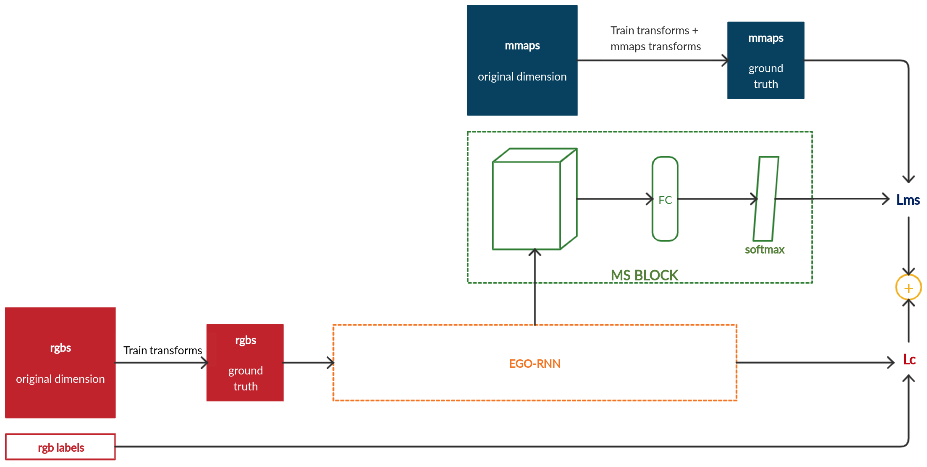
\includegraphics[width=\linewidth]{images/egornn+msblock_architecture.png}
  \caption{Generic architecture of motion segmentation branch applied to \textit{egornn}}
  \label{msblock_arch}
\end{figure*}

\subsubsection{MS task as regression}

A possible variation of this task was to implement this self-supervised task as a regressor. In this way, the network output is not anymore a softmax unit that estimates the probability of the possible classes, but is now a single value for each pixel interpreted as the mean of a conditional gaussian

\begin{align*}
\hat{y} = W^Th + b\\
p(y|x) = N(y; \hat{y},I)\\
\end{align*}

Where $\hat{y}$ is the linear output units. In this case maximizing the log-likelihood corresponds to minimizing the mean squared error in the training data, so we switched to a Squared Error loss for this task.

\begin{align*}
\hat{y} = W^Th + b\\
L(y - \hat{y}) = \sum_{i=1}^{n}(y_i - \hat{y_i})^2
\end{align*}

After summing the squared errors in our batch, we divide again by batch size and number of frames to get the mean error on a single map.

\subsubsection{Our variation on the MS task}

Analyzing and comparing the results of this architecture with the one of \cite{egornn} what we found is that even though it did improve the motion embedding into the features and we show this in the experiments section. Though one thing that this model actually suffered from was the lack of precision in the spatial localisation of motion. For example, looking at misclassified examples, we saw that often an action was mistaken for another if it involved grabbing objects that were close to each other. We argue that a a possible solution to counteract on this, is to move the self-supervised block to the \textit{con3} and \textit{con4} outputs of the CNN backbone. Experimenting with this we found that there actually is a trade of, since the network can definitely benefit from having a finer granularity in the motion maps, but if this map is applied to more low-level features, the representation loses some of its power since there are many more features who are being moved around, and probably a part of that motion is just due to camera shiftings. So trying to get the most efficient trade-of between high-level features, and resolution of the maps, we found that implementing the self-supervised task as a regressor applied at \textit{conv4}, so with 14x14 maps, can
be actually quite helpful and achieve a 10 percent performance boost using only 7 frames with respect to the baseline with same number of frames.
We chose the regressor over the classifier for the ms block since it gives us the possibility of applying a little trick. Using regression we can obtain the ground truth, instead of downsampling, by taking the mean of the square around the pixel of interest. In this way our ground truths are not anymore binary but actually a grayscale ranging from \textit{static} (0) and \textit{moving} (1).


\subsection{Static-dynamic discriminator}

Our previous variations of increasing the resolution of the MS task stemmed from the observation that
the model suffered from a lack of precision in identifying the motion location. Even with that modifications, the network still had problems in completely discerning between symmetrical actions, like open/close objects. The architecture that we propose to improve upon this situation includes a discriminator at the end of the convLSTM module, trained to discern amongst 2 classes :\textit{static} and \textit{dynamic}. The idea is, instead of struggling to extract feature that encode motion from RGB frames
in a CNN which is not built to encode temporal differences, move this task to the convLSTM module,
which natively has the capability of representing features that evolve through time. This discriminator is trained jointly with the rest of the network, and is fed with 2 types of inputs:
- a first forward pass consisting of the actual output of the CNN, for all frames, labeled as \textit{dynamic}
- a second forward pass using n (with n number of frames) times the same feature map.
The idea is that in this way the discriminator should penalyze the features that do not encode
any motion information, and privilege the others, resulting in a model that is better able to
keep track of motions.
This task is implemented as a simple binary classification problem with again a Cross Entropy Loss.
The final minimization problem, which also includes the MS task from \cite{sparnet}, is the following,
where $t$ is the label of this new discriminator $t \in {\textit{static}, \textit{dynamic}}$ ,
$\theta_d$ represents the discriminator classification space, and the rest of the notations is the same as
before. The resulting loss to minimize in reported in the last row, and includes weighting parameter $\alpha$ to adjust the importance to give to the discriminator.

\begin{align*}
L_c(x,y) &= - \sum_{i=1}^{n} y_i log(p(y|x, \theta_c, \theta_f))\\
L_d(x,t) &= - \sum_{i=1}^{n} t_i log(p(t|x, \theta_d, \theta_f))\\
L_{ms}(x,m) &= - \sum_{i=1}^{n} \sum_{k=1}^{N} \sum_{j=1}^{s^2} m_i^k(j)log(l_i^k(j))
\end{align*}
\begin{align*}
L(x,y,m,t| \theta_M) &= L_c(x,y|\theta_f, \theta_c) + \\
&+ L_{ms}(x,m| \theta_f, \theta_{ms} + \\
&+ \alpha L_d(x,t| \theta_f, \theta_{d}  )
\end{align*}

Even though this approach was not able to improve upon our baseline, it did not perform
badly ad we report it anyway as it is an elegant and simple solution that may turn out to be useful in cases other than our small GTEA61 dataset.

\subsection{Representation Flow layer}
Optical flow can be a source of useful features that encode motion and temporal clues.
The problem though, it's that it requires an expensive optimization procedure to be obtained, and when used as usual in 2 stream networks renders the inference time quite long, besided making more expensive the training.
This idea was based on the works of \cite{motfilt} and \cite{reprflow}. The first one
introduces the idea of estimating the flow from directly from RGB frames inside the CNN layers. The second one improves to procedure, making it a bit heavier computationally, but more powerful, embedding it in a fully-differentiable and learnable layer to include in a CNN backbone. The authors of \cite{reprflow} found that inserting this layer at the input performs as poorly as a flow only networks, whereas placing it after the \textit{conv3} block of the backbone resNet achieves the best result. This approach leverages the
fact that by estimating flow on a feature map which is low resolution compared to a full images allows to slim the computational cost, and since it is learned in an end-to-end fashion in the training pipeline, is able to extract motion informations that are more related to the features, and so are even better than the standard optical flow. \reff{flow2} reports the formal procedure with which the differentiable layer implements the flow estimation, whereas \reff{flow1} represents their proposed architecturs.
In \cite{reprflow} they apply this to a a CNN backbone, and to a 3D version of it. We argue that including this layer even if it is able to associate the motion information to the feature map that the network extracts, is still lacking a spatio-temporal mapping of the evolution of the features throghout a video. For this reason we included it in
our architecture in the following way.
We take our frames through the first 3 residual blocks of our ResNet34 backbone, then
we apply the proposed layer to estimate the optical flow from the features map, and then
we forward them to the rest of the CNN and afterwards to the convLSTM module. In
this scenario we deactivate the spatial attention mechanism, as it was oriented to
highlight regions based on the static appearance, and not to work with more motion-oriented features.

\begin{figure*}
  \centering
  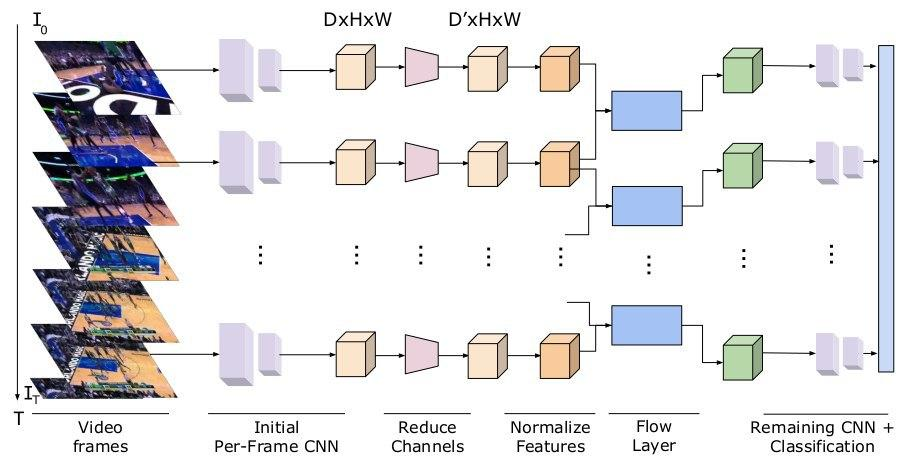
\includegraphics[width=.7\linewidth]{images/flow1.jpg}
  \caption{Illustration of a video-CNN with the representation flow layer. The CNN computes intermediate feature maps, that are used as input to the flow layer. The outputs of  are used for prediction.}
  \label{flow1}
\end{figure*}
\begin{figure}[t]
  \centering
  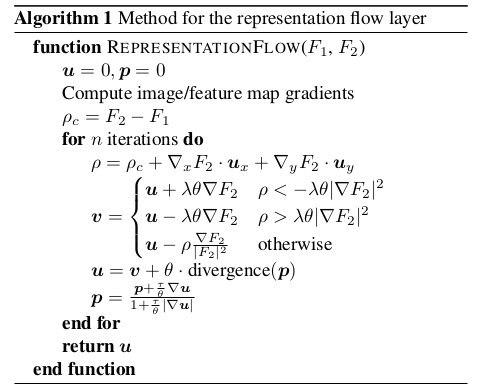
\includegraphics[width=\linewidth]{images/flow2.jpg}
  \caption{Algorithm to extract optical flow from feature maps of the CNN}
  \label{flow2}
\end{figure}


\subsection{Dataset description}

The dataset under analysis is a modified version of GTEA61\footnote{Georgia Tech Egocentric Activity Datasets: \small{\url{http://cbs.ic.gatech.edu/fpv/}}}. The dataset contains the videos in form of frames, and also two kind of preprocessed images: \textit{motion maps} and \textit{optical flows}. The folder schema of the dataset is shown in \reff{folder_schema}. Videos represent 61 class actions performed by 4 different users (\textit{S1}, \textit{S2}, \textit{S3}, \textit{S4}). Sometimes for some actions more than one video is available. The total number of videos in the dataset is, however, 457, which actually means that it is a quite small dataset.

\begin{figure*}
	\centering
	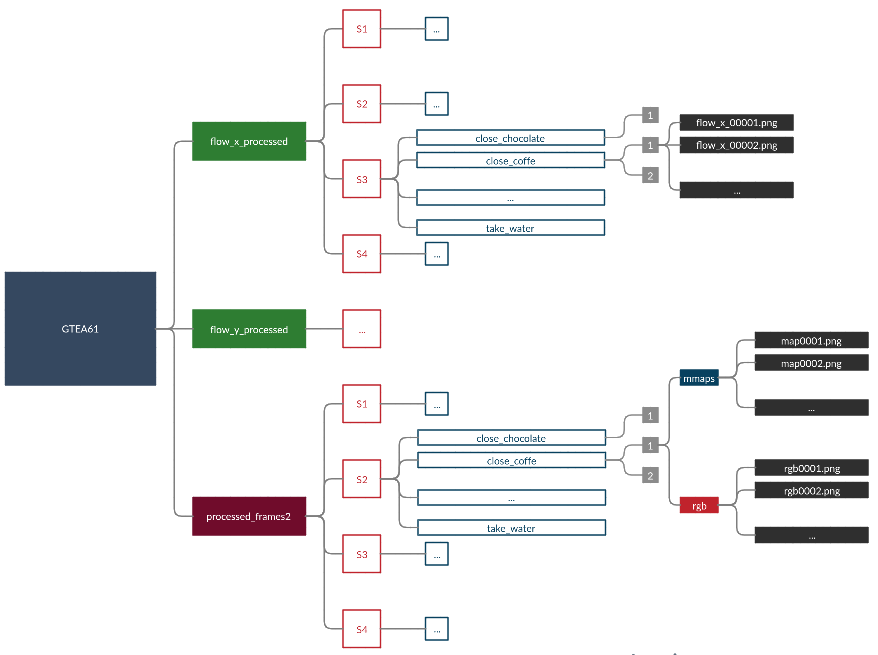
\includegraphics[width=.9\linewidth]{images/folder_schema.png}
	\caption{Folder schema of our GTEA61}
	\label{folder_schema}
\end{figure*}

The optical flow methods try to calculate the motion between two image frames which are taken at times $t$ and $t + \Delta t$ at every voxel position. The warp flow methods try also to remove the motion of the wearable camera. We have two kind of these last representations in our dataset: one computed in the horizontal axis (folder \textit{flow\_x\_processed}) and one other computed in the vertical axis (folder \textit{flow\_y\_processed}).

The motion maps are special black-and-white images which represent the spatial location in which the Motion Segmentation task of \cite{sparnet} focuses its attention per each frame. The mmaps present large similarities with the warp flows.

The differences between the kind of available images in our dataset are shown in \reff{image_comparison}.

\begin{figure*}
  \centering
  \begin{subfigure}{.24\linewidth}
  	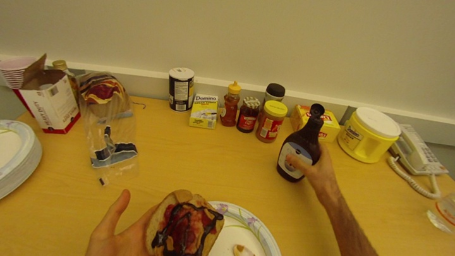
\includegraphics[width=\linewidth]{images/img_comp/rgb0001.png}
  \end{subfigure}
  \begin{subfigure}{.24\linewidth}
  	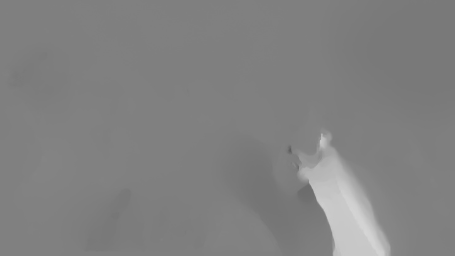
\includegraphics[width=\linewidth]{images/img_comp/flow_x_00002.png}
  \end{subfigure}
  \begin{subfigure}{.24\linewidth}
  	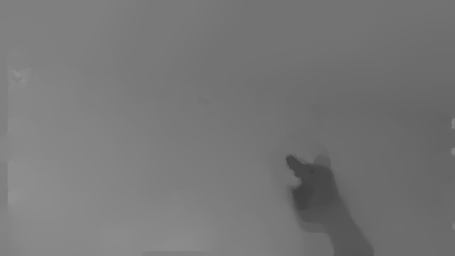
\includegraphics[width=\linewidth]{images/img_comp/flow_y_00001.png}
  \end{subfigure}
  \begin{subfigure}{.24\linewidth}
  	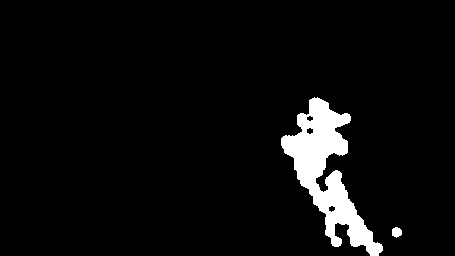
\includegraphics[width=\linewidth]{images/img_comp/map0001.png}
  \end{subfigure}
  \begin{subfigure}{.24\linewidth}
  	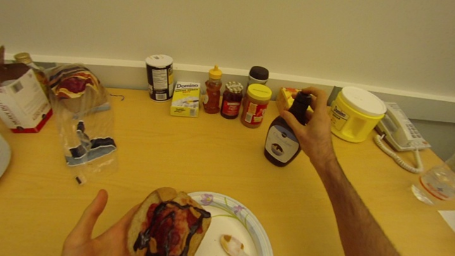
\includegraphics[width=\linewidth]{images/img_comp/rgb0011.png}
  \end{subfigure}
  \begin{subfigure}{.24\linewidth}
  	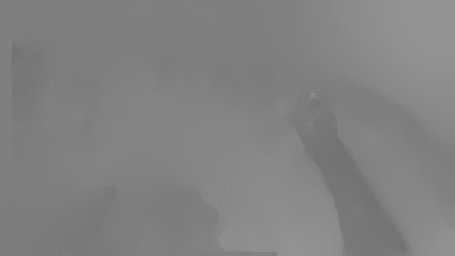
\includegraphics[width=\linewidth]{images/img_comp/flow_x_00011.png}
  \end{subfigure}
  \begin{subfigure}{.24\linewidth}
  	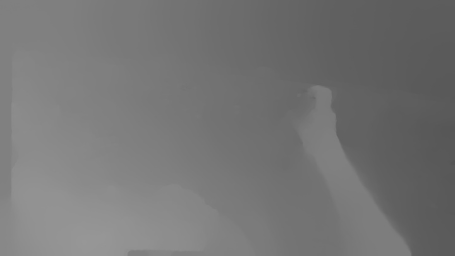
\includegraphics[width=\linewidth]{images/img_comp/flow_y_00011.png}
  \end{subfigure}
  \begin{subfigure}{.24\linewidth}
  	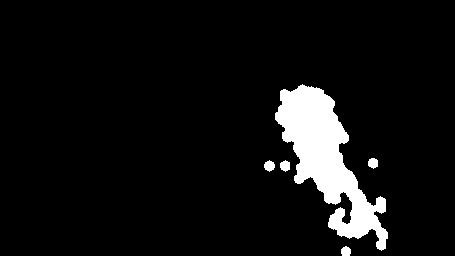
\includegraphics[width=\linewidth]{images/img_comp/map0011.png}
  \end{subfigure}
  \begin{subfigure}{.24\linewidth}
  	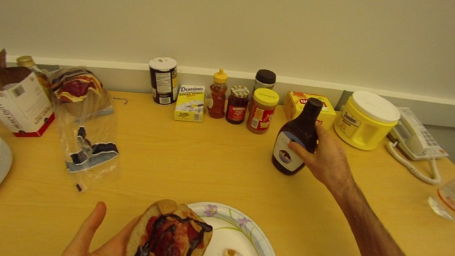
\includegraphics[width=\linewidth]{images/img_comp/rgb0020.png}
  \end{subfigure}
  \begin{subfigure}{.24\linewidth}
  	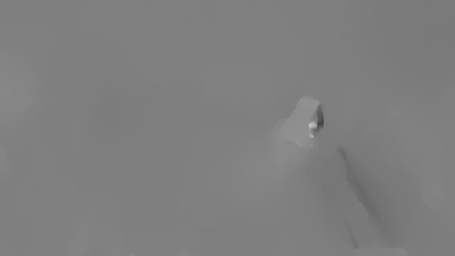
\includegraphics[width=\linewidth]{images/img_comp/flow_x_00020.png}
  \end{subfigure}
  \begin{subfigure}{.24\linewidth}
  	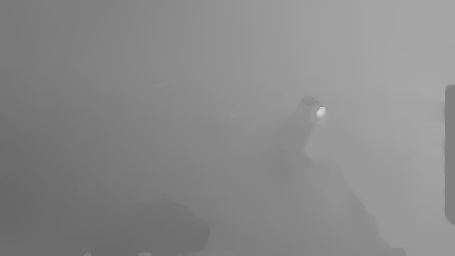
\includegraphics[width=\linewidth]{images/img_comp/flow_y_00020.png}
  \end{subfigure}
  \begin{subfigure}{.24\linewidth}
  	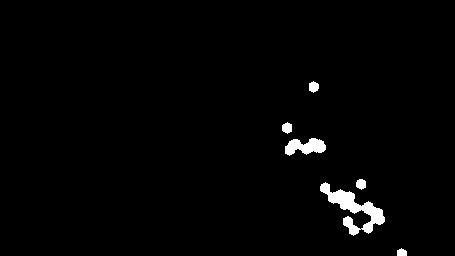
\includegraphics[width=\linewidth]{images/img_comp/map0020.png}
  \end{subfigure}
  \caption{Types of images in our dataset. In this example is shown a sample of images from the \textit{close\_chocolate} action. From the left column to the right column: rgbs, warp flows x, warp flows y, motion maps}
  \label{image_comparison}
\end{figure*}

\subsection{Data cleaning}

The dataset was almost clean already from the beginning, but we encountered two problems within it:
\begin{itemize}
  \item there were hidden useless folders \textit{.DSstore} inside each one of the user folders. These have been removed
  \item some of the first mmaps of some videos were missing. In these cases we have simply duplicated the second mmap
\end{itemize}


\section{Experiments}

Our nets are always trained on a predefined train set, which includes all and only the videos of the users \textit{S1}, \textit{S3} and \textit{S4}, while validation and test sets coincide and is constituted by all and only the videos of a single user, \textit{S2}. In addition, the weights of the \textit{resnet34} are pretrained on ImageNet. Each model is always validated while it is trained, so for each training phase we selected the weights with the highest accuracy at a particular epoch as the best ones.

Due to Colab limitations of GPU memory, we have only been able to perform experiments on a limited amount of frames (7 or, in less cases, 16). Due to this problem our results should be interpreted not as absolute value of the accuracy, but as a sort of relative value with respect to the number of frames for each video in our batches.

The size of our batches has always been left to 32, as well as the number of hidden units of the convLSTM module, fixed at 512. Our optimization algorithm is always Adaptive moment estimation (ADAM) with the only exception of \textit{flow\_resnet34}, for which it is Stochastic Gradient Descent (SGD). When using this last optimizer, the momentum has always been left to 0.9. The scheduler is a MultiStepLR scheduler, which decreases the original learing rate LR by a factor GAMMA at each value of STEP\_SIZE.

\subsection{Egornn}

We have replied some of the same experiments of \cite{egornn} on the original egornn. We have run each of these experiments three times and then we have averaged the results.

First, we have performed the classification by using the \textit{egornn} without and with the CAM. The training phase has been divided in two parts, as in the original paper:

\begin{enumerate}
  \item train of ConvLSTM and Classifier (green blocks in \reff{egornn_arch})
  \item train of conv5 (layer4 of \textit{resnet34}), FC(1000), Spatial Attention Layer (orange blocks in \reff{egornn_arch}) in addition to the previously listed blocks
\end{enumerate}

The values of the hyperparameters for the first stage are:

\begin{center}
	\setstretch{1}
  \scalebox{0.7}{
  	\begin{tabular}{|c|c|}
  		 \hline
  		 \textbf{LR} & 1e-3 \\
  		 \hline
  		 \textbf{WEIGHT\_DECAY} & 4e-5 \\
  		 \hline
  		 \textbf{NUM\_EPOCHS} & 200 \\
  		 \hline
  		 \textbf{STEP\_SIZE} & [25, 75, 150] \\
  		 \hline
  		 \textbf{GAMMA} & 0.1 \\
  		 \hline
  	\end{tabular}
  }
	\setstretch{0.1}
\end{center}

While, for the second stage, they are:

\begin{center}
	\setstretch{1}
  \scalebox{0.7}{
  	\begin{tabular}{|c|c|}
  		 \hline
  		 \textbf{LR} & 1e-4 \\
  		 \hline
  		 \textbf{WEIGHT\_DECAY} & 4e-5 \\
  		 \hline
  		 \textbf{NUM\_EPOCHS} & 150 \\
  		 \hline
  		 \textbf{STEP\_SIZE} & [25, 75] \\
  		 \hline
  		 \textbf{GAMMA} & 0.1 \\
  		 \hline
  	\end{tabular}
  }
	\setstretch{0.1}
\end{center}

Then, we have also trained \textit{flow\_resnet34} alone. In this case we used only 5 frames per each flow (x and y) due to the fact that for some videos no more than 5 frames were provided.

The values of the hyperparameters in this case are:

\begin{center}
	\setstretch{1}
  \scalebox{0.7}{
  	\begin{tabular}{|c|c|}
  		 \hline
  		 \textbf{LR} & 1e-2 \\
  		 \hline
  		 \textbf{WEIGHT\_DECAY} & 5e-4 \\
  		 \hline
  		 \textbf{NUM\_EPOCHS} & 750 \\
  		 \hline
  		 \textbf{STEP\_SIZE} & [150, 300, 500] \\
  		 \hline
  		 \textbf{GAMMA} & 0.5 \\
  		 \hline
  	\end{tabular}
  }
	\setstretch{0.1}
\end{center}

At last we performed the two stream training with the following values for the hyperparameters:

\begin{center}
	\setstretch{1}
  \scalebox{0.7}{
  	\begin{tabular}{|c|c|}
  		 \hline
  		 \textbf{LR} & 1e-2 \\
   		 \hline
   		 \textbf{LR\_FLOW} & 1e-4 \\
  		 \hline
  		 \textbf{WEIGHT\_DECAY} & 5e-4 \\
  		 \hline
  		 \textbf{NUM\_EPOCHS} & 250 \\
  		 \hline
  		 \textbf{STEP\_SIZE} & [1] \\
  		 \hline
  		 \textbf{GAMMA} & 0.99 \\
  		 \hline
  	\end{tabular}
  }
	\setstretch{0.1}
\end{center}

Where LR is the learning rate of \textit{egornn} and LR\_FLOW is the learning rate of \textit{flow\_resnet34}.

The summary of our results is shown in \reff{step1_table}.  From here it raises that the best model is the two-stream (joint train) with 16 frames, followed by EGO-RNN - stage 2 with 16 frames, which is behind the two-stream model by less than 1 point of mean accuracy. Due to the averaging between three identical runs we can rely on this result and assert that the contribution of \textit{flow\_resnet34} slightly increases the performances, but also that the most of the contribution is given by \textit{egornn}.

\begin{figure}[t]
	\centering
	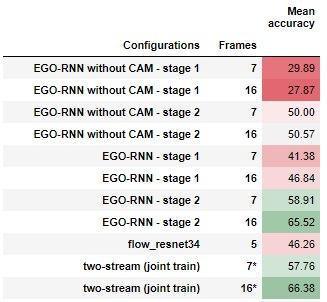
\includegraphics[width=\linewidth]{images/step1_table.jpg}
	\caption{Summary of the results over different configurations. Each value of the mean accuracy is the mean of the accuracies over three identical experiments. \small{*the number of frames refers to the \textit{egornn} branch (for the flow\_resnet34 branch the number of frames is always 5)}}
	\label{step1_table}
\end{figure}

In \reff{step1_acc} and \reff{step1_loss} are shown respectively the validation accuracy and the validation loss by epoch of one random extracted run per each one of the attempts with 16 frames (5 in case of \textit{flow\_resnet34}) and only for the stage 2 when a two stage training is requiered.

\begin{figure}[t]
	\centering
	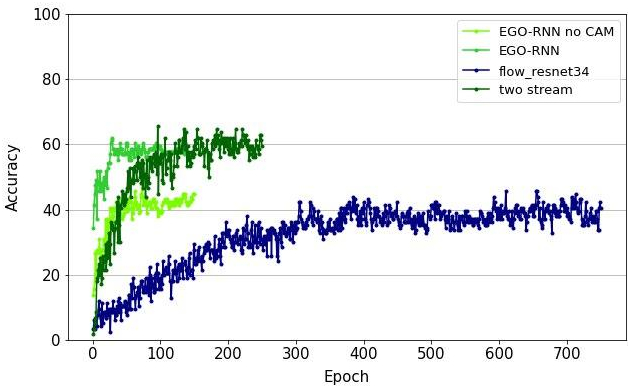
\includegraphics[width=\linewidth]{images/step1_acc.jpg}
	\caption{Validation accuracy by epoch of one random extracted run for the four most interesting training configurations}
	\label{step1_acc}
\end{figure}

\begin{figure}[t]
	\centering
	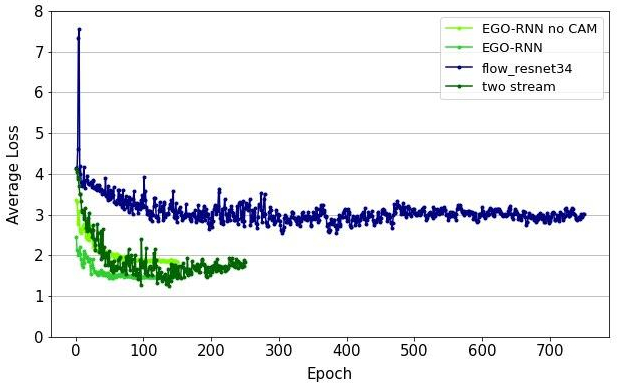
\includegraphics[width=\linewidth]{images/step1_loss.jpg}
	\caption{Validation loss by epoch of one random extracted run for the four most interesting training configurations. The losses are the average of each batch loss within a single epoch}
	\label{step1_loss}
\end{figure}

From \reff{step1_acc} and \reff{step1_loss} is even more evident that \textit{flow\_resnet34} is highly inefficient alone, and that the results with the CAM are heavily better than the results without the CAM (higher accuracy and lower loss at every epoch). The two-stream model requieres more time to get high accuracies, and overall it seems to have the same behaviour of \textit{egornn} when at full capacity, but it is noisier and so it is easier that for some epoch the accuracy is higher.

In \reff{cams1_1} and \reff{cams1_2} are shown the CAMs from a couple of video frames exctracted from \textit{egornn}. As we can observe, the precision is not so high: the CAM often miss to focus on the motion.

\begin{figure}[t]
  \centering
  \begin{subfigure}{.35\linewidth}
  	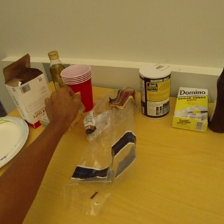
\includegraphics[width=\linewidth]{images/Cams1/S2_take_cheese/rgb0020.png}
  \end{subfigure}
  \begin{subfigure}{.35\linewidth}
  	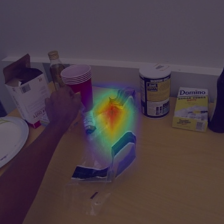
\includegraphics[width=\linewidth]{images/Cams1/S2_take_cheese/rgb0020_CAM.png}
  \end{subfigure}
  \begin{subfigure}{.35\linewidth}
  	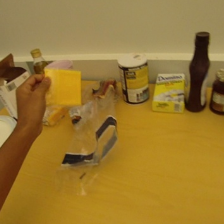
\includegraphics[width=\linewidth]{images/Cams1/S2_take_cheese/rgb0027.png}
  \end{subfigure}
  \begin{subfigure}{.35\linewidth}
  	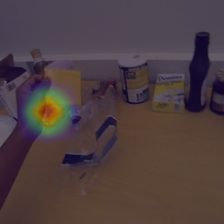
\includegraphics[width=\linewidth]{images/Cams1/S2_take_cheese/rgb0027_CAM.png}
  \end{subfigure}
  \caption{Example of CAMs from take\_cheese action}
  \label{cams1_1}
\end{figure}

\begin{figure}[t]
  \centering
  \begin{subfigure}{.35\linewidth}
  	\includegraphics[width=\linewidth]{images/Cams1/S2_take_honey/rgb0004.png}
  \end{subfigure}
  \begin{subfigure}{.35\linewidth}
  	\includegraphics[width=\linewidth]{images/Cams1/S2_take_honey/rgb0004_CAM.png}
  \end{subfigure}
  \begin{subfigure}{.35\linewidth}
  	\includegraphics[width=\linewidth]{images/Cams1/S2_take_honey/rgb0007.png}
  \end{subfigure}
  \begin{subfigure}{.35\linewidth}
  	\includegraphics[width=\linewidth]{images/Cams1/S2_take_honey/rgb0007_CAM.png}
  \end{subfigure}
  \caption{Example of CAMs from take\_honey action}
  \label{cams1_2}
\end{figure}


\subsection{Motion Segmentation branch applied to egornn}

The wrong focus of the CAMs  highly justifies the implementation of the self-supervised task which exploits the motion maps. First of all we have replied the same experiment of \cite{sparnet} (the one in which \textit{egornn} is the Action Recognition Block). The hyperparameters used are:

\begin{center}
	\setstretch{1}
  \scalebox{0.7}{
  	\begin{tabular}{|c|c|}
  		 \hline
  		 \textbf{LR} & 1e-3 \\
   		 \hline
  		 \textbf{WEIGHT\_DECAY} & 4e-5 \\
  		 \hline
  		 \textbf{NUM\_EPOCHS} & 150 \\
  		 \hline
  		 \textbf{STEP\_SIZE} & [50, 100] \\
  		 \hline
  		 \textbf{GAMMA} & 0.1 \\
  		 \hline
  	\end{tabular}
  }
	\setstretch{0.1}
\end{center}

for the stage1, while they are the following:

\begin{center}
	\setstretch{1}
  \scalebox{0.7}{
  	\begin{tabular}{|c|c|}
  		 \hline
  		 \textbf{LR} & 1e-4 \\
   		 \hline
  		 \textbf{WEIGHT\_DECAY} & 4e-5 \\
  		 \hline
  		 \textbf{NUM\_EPOCHS} & 150 \\
  		 \hline
  		 \textbf{STEP\_SIZE} & [25, 75] \\
  		 \hline
  		 \textbf{GAMMA} & 0.1 \\
  		 \hline
  	\end{tabular}
  }
	\setstretch{0.1}
\end{center}

for the stage2. We have decreased the number of epochs for the stage1 because we have observed that going too far with the epochs, with the loss decreased after the steps of the optimizer, would be meaningless and does not give any significant result.

The results with the same values for the hyperparameters are shown in \reff{ms_table}.

\begin{figure}[t]
	\centering
	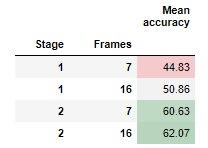
\includegraphics[width=.6\linewidth]{images/step2.1_table.jpg}
	\caption{Mean accuracies over three identical experiments with the same fixed set of values for the hyperparameters, by varying only the stage of training and the number of frames - classification experiment}
	\label{ms_table}
\end{figure}

As expected, the best performances are achieved after the second stage of training and with 16 frames.

We have also replied this experiment as a regression problem.
[REGRESSION IMPLEMENTATION]

In \reff{ms_reg_table} are shown the results.

\begin{figure}[t]
	\centering
	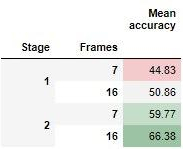
\includegraphics[width=.52\linewidth]{images/step2.3_table.jpg}
	\caption{Mean accuracies over three identical experiments with the same fixed set of values for the hyperparameters, by varying only the stage of training and the number of frames - regression experiment}
	\label{ms_reg_table}
\end{figure}

Also in this case the highest value of the accuracy is obtained for 16 frames. The first stage is exactly the same so we have not replied it three times more. For the second stage we observe that with this combination of values for the hyperparameters the regression performs more than 4 points better than classification with 16 frames, while the accuracies are roughly the same when the number of frames is 7.

We have performed also a complete grid search to improve the performances of the net.

Before starting, it has been execuded a brief tuning step for the stage 1 of training, which is the same for both the classification and the regression methodologies. The values of interest have been STEP\_SIZE and GAMMA only. From this we obtained that the optimal values for the stage1 are exaclty the same used in the previous experiment.

After this preliminary step, the complete grid search has been executed only on the stage 2, which is the most important one. The number of selected frames is 16, for which we have seen that the performances are better than for 7. We have reduced NUM\_EPOCHS to 100 to save computational time (in addition the highest accuracy is rarely obtained after epoch 100). For the classification strategy the results are shown in \reff{ms_grid}, while for the regression they are shown in \reff{ms_reg_grid}.

\begin{figure}[t]
	\centering
	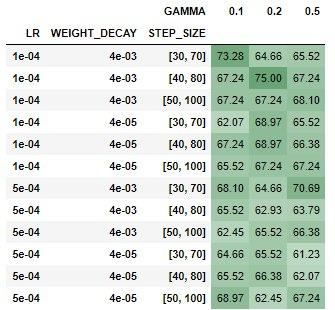
\includegraphics[width=\linewidth]{images/grid_no_reg_table.jpg}
	\caption{Accuracies at various combinations of hyperparameters for the classification strategy}
	\label{ms_grid}
\end{figure}

\begin{figure}[t]
	\centering
	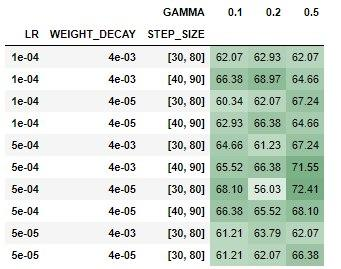
\includegraphics[width=\linewidth]{images/grid_reg_table.jpg}
	\caption{Accuracies at various combinations of hyperparameters for the regression strategy}
	\label{ms_reg_grid}
\end{figure}

As we can observe the best performances are achieved with:
\begin{itemize}
  \item $LR = 10^{-4}, WEIGHT\_DECAY = 4 \cdot 10^{-3}, STEP\_SIZE = [40, 80]$ for the classification method, for an accuracy of 75.00
    \item $LR = 5 \cdot 10^{-4}, WEIGHT\_DECAY = 4 \cdot 10^{-5}, STEP\_SIZE = [30, 80]$ for the regression method, for an accuracy of 72.41
\end{itemize}

In general we can say that the performances are better with the classification method, and this is a surprisingly result based on the observations without the grid. The reason for the previous result was that, as emerges from \reff{ms_grid} and \reff{ms_reg_grid}, the optimal values for the hyperparameters falls in a total different region with respect to the two different methodologies.

In \reff{grid_comparison} we can observe the effects of the values of the hyperparameters on the accuracy and on the loss of both train and validation and over three different experiments present in the grid search with the classification methodology. The colors of the graphs underline the different learning rate before ad after each step of the optimizer. The steps are shown on the x axis and marked with a vertical gray line. In (a) is shown the best result obtained, while (b) and (c) are representative examples with different tuned values for the hyperparameters. In (a) the loss already starts from a low value and the accuracy already starts from an high value. LR highly influences the starting point of the accuracy and the loss in epoch 1 (higher LR $\rightarrow$ lower initial accuracy and higher initial loss). To show this behaviour it has been picked the example in (b), which has the same STEP\_SIZE but different values for the other hyperparameters. We can observe that, from \reff{ms_grid}, there is not a tangible difference between the column with GAMMA = 0.1 and the column with GAMMA = 0.2, while it is more evident that with GAMMA = 0.5 the accuracy worsen a bit. So, it has been selected another example, (c),  with GAMMA = 0.1 (which is a different gamma with respect to (a)) and the same values of LR and WEIGHT\_DECAY (which differs from (a)), and with another STEP\_SIZE. The effect of this slight variation on the STEP\_SIZE seems to be not so meaningful, while the actual main characters of the different behaviour of the net are LR and WEIGHT\_DECAY, together with GAMMA which is good when it is 0.1 as well as when in is 0.2. As last observations:
\begin{itemize}
  \item is evident from all the three experiments that the train accuracy continue growing also when the validation accuracy starts flattening, and the behaviour is the relative one for the loss
  \item both the losses and the accuracies are \quotes{noisier} when the learning rate is higher
  \item the global behaviour is strongly influenced by the random batches which feed the net, and so the results should be intended within an error margin
\end{itemize}

\begin{figure*}
  \centering
  \captionsetup[subfigure]{justification=centering}
  \begin{subfigure}{.325\linewidth}
  	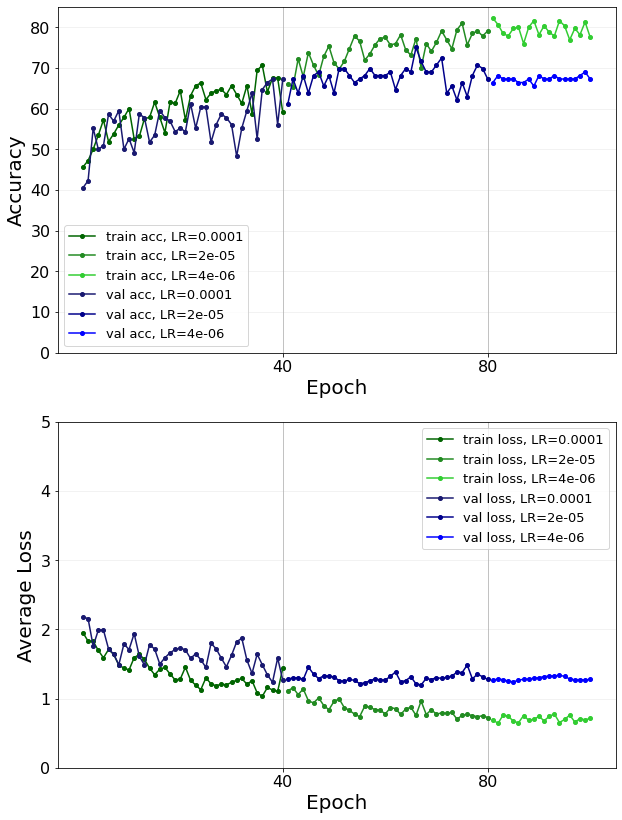
\includegraphics[width=\linewidth]{images/grid_comparison/acc75no_reg.png}
    \subcaption{\\LR = 1e-4\\WEIGHT\_DECAY = 4e-3\\STEP\_SIZE = [40, 80]\\GAMMA = 0.2\\Highest accuracy = 75.00\\at epoch 66}
  \end{subfigure}
  \begin{subfigure}{.325\linewidth}
  	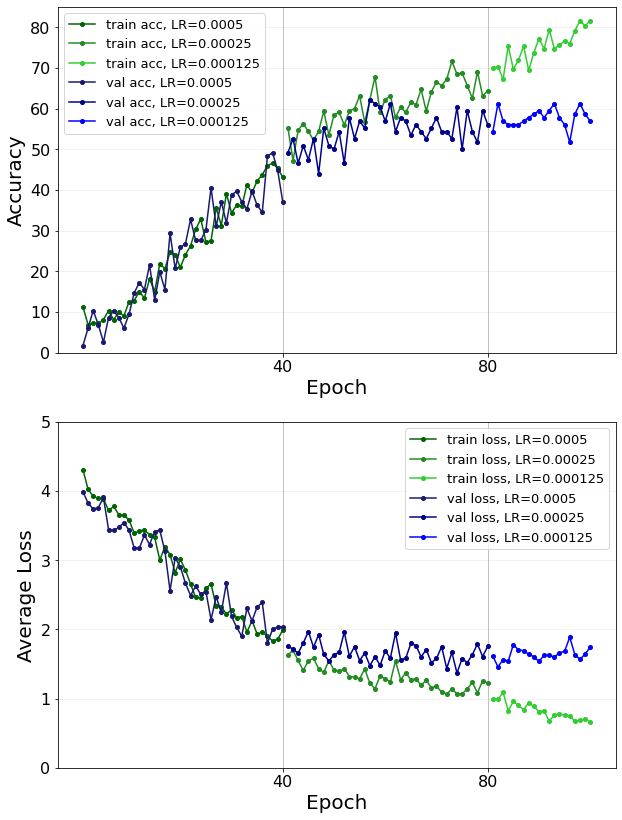
\includegraphics[width=\linewidth]{images/grid_comparison/acc62lr5e-4step4080gamma05_no_reg.png}
    \subcaption{\\LR = 5e-4\\WEIGHT\_DECAY = 4e-5\\STEP\_SIZE = [40, 80]\\GAMMA = 0.5\\Highest accuracy = 62.07\\at epoch 57}
  \end{subfigure}
  \begin{subfigure}{.325\linewidth}
  	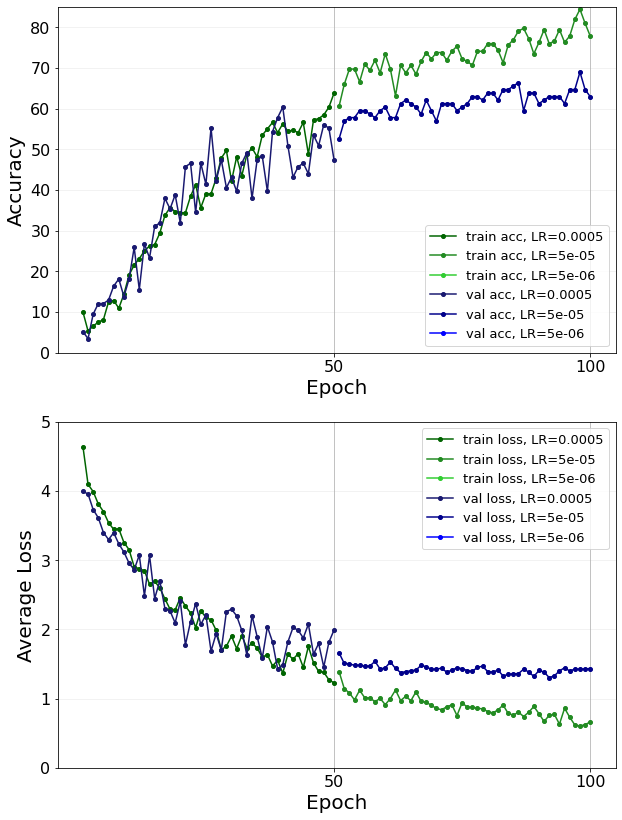
\includegraphics[width=\linewidth]{images/grid_comparison/acc69lr5e-4step50100gamma01_no_reg.png}
    \subcaption{\\LR = 5e-4\\WEIGHT\_DECAY = 4e-5\\STEP\_SIZE = [50, 100]\\GAMMA = 0.1\\Highest accuracy = 68.97\\at epoch 98}
  \end{subfigure}
  \caption{Comparison between three representative experiments in the grid search with the classification method\\}
  \label{grid_comparison}
\end{figure*}

Finally, we can observe examples of CAMs generated by this kind of experiments in \reff{cam2_1} and \reff{cam2_2}.

\begin{figure}[t]
  \centering
  \begin{subfigure}{.32\linewidth}
  	\includegraphics[width=\linewidth]{images/Cams2/S2_take_honey/rgb0004.png}
  \end{subfigure}
  \begin{subfigure}{.32\linewidth}
  	\includegraphics[width=\linewidth]{images/Cams2/S2_take_honey/rgb0004_CAM.png}
  \end{subfigure}
  \begin{subfigure}{.32\linewidth}
  	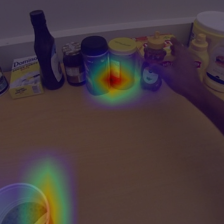
\includegraphics[width=\linewidth]{images/Cams2/S2_take_honey/rgb0004_CAM_MS.png}
  \end{subfigure}
  \begin{subfigure}{.32\linewidth}
  	\includegraphics[width=\linewidth]{images/Cams2/S2_take_honey/rgb0007.png}
  \end{subfigure}
  \begin{subfigure}{.32\linewidth}
  	\includegraphics[width=\linewidth]{images/Cams2/S2_take_honey/rgb0007_CAM.png}
  \end{subfigure}
  \begin{subfigure}{.32\linewidth}
  	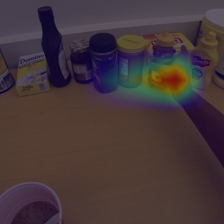
\includegraphics[width=\linewidth]{images/Cams2/S2_take_honey/rgb0007_CAM_MS.png}
  \end{subfigure}
  \caption{Example of CAMs from take\_honey action generated with \textit{egornn} with the Motion Segmentation Branch. the cams shown in the center are without MS Block, the CAMs on the right are with the MS Block}
  \label{cam2_1}
\end{figure}

\begin{figure}[t]
  \centering
  \begin{subfigure}{.32\linewidth}
  	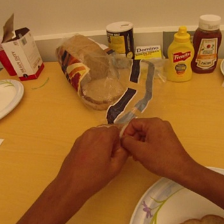
\includegraphics[width=\linewidth]{images/Cams2/S2-take_hotdog/rgb0057.png}
  \end{subfigure}
  \begin{subfigure}{.32\linewidth}
  	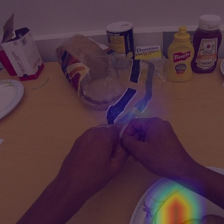
\includegraphics[width=\linewidth]{images/Cams2/S2-take_hotdog/rgb0057_CAM.png}
  \end{subfigure}
  \begin{subfigure}{.32\linewidth}
  	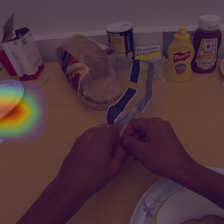
\includegraphics[width=\linewidth]{images/Cams2/S2-take_hotdog/rgb0057_CAM_MS.png}
  \end{subfigure}
  \begin{subfigure}{.32\linewidth}
  	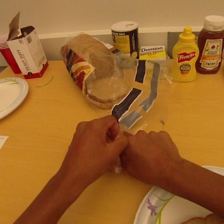
\includegraphics[width=\linewidth]{images/Cams2/S2-take_hotdog/rgb0076.png}
  \end{subfigure}
  \begin{subfigure}{.32\linewidth}
  	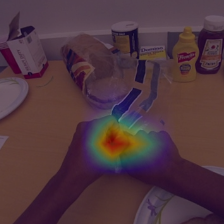
\includegraphics[width=\linewidth]{images/Cams2/S2-take_hotdog/rgb0076_CAM.png}
  \end{subfigure}
  \begin{subfigure}{.32\linewidth}
  	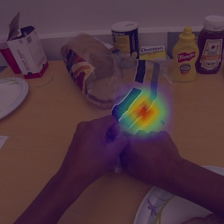
\includegraphics[width=\linewidth]{images/Cams2/S2-take_hotdog/rgb0076_CAM_MS.png}
  \end{subfigure}
  \caption{Example of CAMs from take\_hotdog action generated with \textit{egornn} with the Motion Segmentation Branch. the cams shown in the center are without MS Block, the CAMs on the right are with the MS Block}
  \label{cam2_2}
\end{figure}

From these CAMs we can see that the Motion Segmentation Block helps to focus on the movements, but it is sometimes still inaccurate.

\subsection{New experiments}

\subsubsection{The problem of the Motion Maps}

The CAMs suggested to us to go in deep with the analysis of the motion maps, trying to improve the attention of the net.

To assert if there is an actual contribution of the Motion Segmentation branch and how much it is significant for the final accuracy we analyzed the loss on the mmaps with a special attention. An example of this loss is shown in \reff{loss_mmaps}, which is highly representative because we have observed from several graphs that the behaviour of this loss is always the same. As we can see, the loss on the train set stops to slightly drop after a bunch of epochs.

\begin{figure}[t]
  \centering
  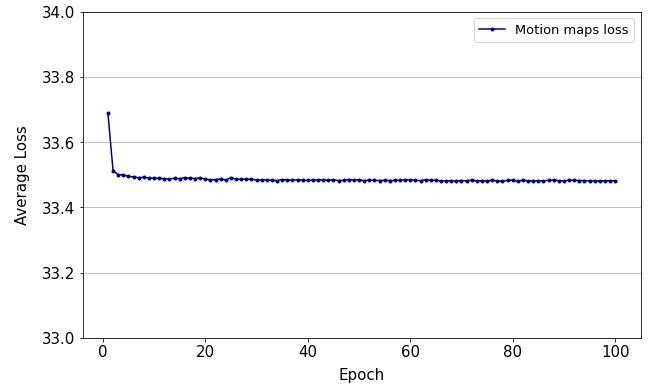
\includegraphics[width=\linewidth]{images/mmaps_loss.jpg}
  \caption{An example of the loss on the classification of the pixels of the downsampled mmaps performed by the Motion Segmentation Branch}
  \label{loss_mmaps}
\end{figure}

We better studied this behaviour by analyzing the CAMs.

To overcome these problems we have tried to increase the resolution of the downsampled mmaps and to treat the problem as regression problem or binary classification problem, and various combinations of this. When handling with the regression problem, we have also tried to use different kind of downsampled motion maps, with a simple technique developed by us that we called \textit{grid technique} for the sake of comprehensibility. Our base downsampling technique is inspired by \cite{downsampling}, but we observed that with a brutal downsampling like this one there is an high risk to loss information. For example, we could take a black pixel contoured by white pixels. This is not good for the net and could bring to misclassification. So, we divided the original 224x224 mmap (obtained after the application of the same kind of trasformations applied to the rgbs without the \textit{normalize} transform) in $l$x$l$ blocks of ($224/l$)x($224/l$) pixels, where $l$ is 7, 14 or 28. The corresponding pixel in the final downsampled mmap is the average of the values of the pixels of its block (so, the image becomes a gray scale image). We applied this last kind of downsampling transformation together with only the regression methodology, due to the particular nature of this image (which in so more easily discretizable).

An example of the described images is shown in \reff{mmaps}.

\begin{figure}[t]
	\centering

	\begin{subfigure}{.4\linewidth}
		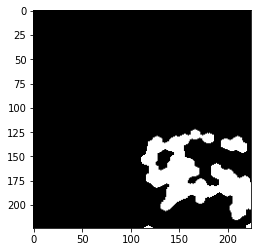
\includegraphics[width=\linewidth]{images/mmaps_example/downsampling224x224_bw.png}
	\end{subfigure}
  \begin{subfigure}{.57\linewidth}
    \begin{subfigure}{.32\linewidth}
  		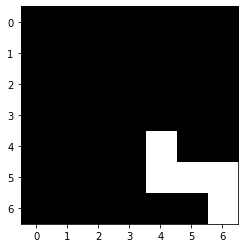
\includegraphics[width=\linewidth]{images/mmaps_example/downsampling7x7_bw.png}
  	\end{subfigure}
  	\begin{subfigure}{.32\linewidth}
  		\includegraphics[width=\linewidth]{images/mmaps_example/downsampling14x14_bw.png}
  	\end{subfigure}
  	\begin{subfigure}{.32\linewidth}
  		\includegraphics[width=\linewidth]{images/mmaps_example/downsampling28x28_bw.png}
  	\end{subfigure}
  	\begin{subfigure}{.32\linewidth}
  		\includegraphics[width=\linewidth]{images/mmaps_example/downsampling7x7_gray.png}
  	\end{subfigure}
  	\begin{subfigure}{.32\linewidth}
  		\includegraphics[width=\linewidth]{images/mmaps_example/downsampling14x14_gray.png}
  	\end{subfigure}
  	\begin{subfigure}{.32\linewidth}
  		\includegraphics[width=\linewidth]{images/mmaps_example/downsampling28x28_gray.png}
  	\end{subfigure}
  \end{subfigure}

	\caption{Example of mmap. In the left: original resolution mmap cropped at 224x224. In the right: from left to right mmaps downsampled at 7x7, 14x14 and 28x28 respectively, from top to bottom mmaps classically downsampled and mmaps generated with the \quotes{grid technique}}
	\label{mmaps}
\end{figure}

To assert which is the best strategy we have trained the net a first time as in the previouses stages 1, with the last set of values for the hyperparameters already showed for stage1, and we have used these weights as starting point for all the stages 2 of the various implementations. The set of hyperparameters chosen for all the implementations for the stages 2 of this section is the following. The choice is based on the observations that we have already done during the grid search analysis, where we have seen that with these values the net performs good.

\begin{center}
	\setstretch{1}
 \scalebox{0.7}{
 	\begin{tabular}{|c|c|}
 		 \hline
 		 \textbf{LR} & 1e-4 \\
  		 \hline
 		 \textbf{WEIGHT\_DECAY} & 4e-5 \\
 		 \hline
 		 \textbf{NUM\_EPOCHS} & 150 \\
 		 \hline
 		 \textbf{STEP\_SIZE} & [30, 80] \\
 		 \hline
 		 \textbf{GAMMA} & 0.2 \\
 		 \hline
 	\end{tabular}
 }
	\setstretch{0.1}
\end{center}

We have performed three experiments for each one of the selected configurations and then averaged the results, as before. The experiments are summarized in \reff{mmaps_table}.

\begin{figure}[t]
  \centering
  \includegraphics[width=.7\linewidth]{images/step3.1_table.jpg}
  \caption{Summary of the mean accuracy values with different combinations of mmaps downsampling techinque and final resolution}
  \label{mmaps_table}
\end{figure}

The first 2 rows of \reff{mmaps_table} act as baseline for our experiments. They are nothing but the experiments proposed in \cite{sparnet}, despite with a lower number of frames due to the already highlighted problems of available memory in Colab. We can observe that:
\begin{itemize}
  \item the regression over the small 7x7 gray-scale mmaps performed slightly worse than with the 7x7 black-and-white mmaps, but still better than the binary classification baseline version. However, this tell us that the regression technique paired with the gray-scale mmaps is not a good imporvement taken alone
  \item increasing the resolution from 7x7 to 28x28 is too much. This is not strongly due to the resolution: higher resolutions should give better results. The problem is that to deal with this high resolution downsampled mmaps we have to extract features from preliminary layers, and this bring us to force the training on more low level layers (conv3) to give sense to the Motion Segmentation branch backward phase of gradients updating
  \item the best trade-off between training the most high level layers possible and to have good high quality representations of the mmaps is for resolution 14x14. Both the techniques performe a lot better then the respective baselines (binary and regression baselines respectively): we get an increase in performances of roughly 7 points of accuracy with respect to the corresponding baseline, which is an awesome result! Considering instead as baseline only the first row, with our best solution we obtained an increase in performances of 13 points of accuracy, which is a substantial improvement!
\end{itemize}

In \reff{cam3_1} and \reff{cam3_2} are shown examples of CAMs like above: these CAMs have been generated with the regression methodology over the gray-scale 14x14 mmaps. These examples show the better recognition of the motion performed by the Spatial Attention Layer when the high level features of \textit{conv4} are updated with the gradients generated by the Motion Segmentation Block trained as regressor, with ground truth motion maps generated with the \textit{grid technique} and with a resolution of 14x14 pixels.

\begin{figure}[t]
  \centering
  \begin{subfigure}{.32\linewidth}
  	\includegraphics[width=\linewidth]{images/Cams3/S2_take_peanut/rgb0004.png}
  \end{subfigure}
  \begin{subfigure}{.32\linewidth}
  	\includegraphics[width=\linewidth]{images/Cams3/S2_take_peanut/rgb0004_CAM.png}
  \end{subfigure}
  \begin{subfigure}{.32\linewidth}
  	\includegraphics[width=\linewidth]{images/Cams3/S2_take_peanut/rgb0004_CAM_MS.png}
  \end{subfigure}
  \begin{subfigure}{.32\linewidth}
  	\includegraphics[width=\linewidth]{images/Cams3/S2_take_peanut/rgb0010.png}
  \end{subfigure}
  \begin{subfigure}{.32\linewidth}
  	\includegraphics[width=\linewidth]{images/Cams3/S2_take_peanut/rgb0010_CAM.png}
  \end{subfigure}
  \begin{subfigure}{.32\linewidth}
  	\includegraphics[width=\linewidth]{images/Cams3/S2_take_peanut/rgb0010_CAM_MS.png}
  \end{subfigure}
  \caption{Example of CAMs from take\_peanut action generated with \textit{egornn} with the Motion Segmentation Branch used with the gray-scale 14x14 motion maps and the regression methodology. The CAMs shown in the center are without MS Block, the CAMs on the right are with the MS Block}
  \label{cam3_1}
\end{figure}

\begin{figure}[t]
  \centering
  \begin{subfigure}{.32\linewidth}
  	\includegraphics[width=\linewidth]{images/Cams3/S2_take_water/rgb0004.png}
  \end{subfigure}
  \begin{subfigure}{.32\linewidth}
  	\includegraphics[width=\linewidth]{images/Cams3/S2_take_water/rgb0004_CAM.png}
  \end{subfigure}
  \begin{subfigure}{.32\linewidth}
  	\includegraphics[width=\linewidth]{images/Cams3/S2_take_water/rgb0004_CAM_MS.png}
  \end{subfigure}
  \begin{subfigure}{.32\linewidth}
  	\includegraphics[width=\linewidth]{images/Cams3/S2_take_water/rgb0011.png}
  \end{subfigure}
  \begin{subfigure}{.32\linewidth}
  	\includegraphics[width=\linewidth]{images/Cams3/S2_take_water/rgb0011_CAM.png}
  \end{subfigure}
  \begin{subfigure}{.32\linewidth}
  	\includegraphics[width=\linewidth]{images/Cams3/S2_take_water/rgb0011_CAM_MS.png}
  \end{subfigure}
  \caption{Example of CAMs from take\_water action generated with \textit{egornn} with the Motion Segmentation Branch used with the gray-scale 14x14 motion maps and the regression methodology. The CAMs shown in the center are without MS Block, the CAMs on the right are with the MS Block}
  \label{cam3_2}
\end{figure}

\subsubsection{Static-dynamic discriminator}
\label{ds_section}
The reasons for this approach are explained in Section \ref{ds_section}. Also here, due to \textit{Colab out of memory errors}, we had to perform the experiments with 7 frames per video instead than with 16. We have tried four different configurations for the training pipeline, each one tried three times to give consistency to the results:
\begin{enumerate}
  \item training of \textit{conv5}, \textit{convLSTM} and the final static-dynamic classifier when forwarding the static frames
  \item training of \textit{convLSTM} and the final static-dynamic classifier when forwarding the static frames
  \item training \textit{convLSTM} and the final static-dynamic classifier when forwarding the static frames. The static-dynamic loss is multiplied by a constant ALPHA = 0.5
  \item training \textit{convLSTM} and the final static-dynamic classifier when forwarding the static frames. The static-dynamic loss is multiplied by a constant ALPHA = 0.1
\end{enumerate}

The reason for the ALPHA constant is to modulate the importance of the Static-dynamic discriminator block.

The Motion Segmentation branch has been used as in \cite{sparnet}, and so the downsampled mmaps are black and white 7x7 resolution mmaps and the technique used is the binary classification one.

The results are shown in \reff{DS_table}.

\begin{figure}[t]
  \centering
  \includegraphics[width=.6\linewidth]{images/step3.2_table.jpg}
  \caption{Summary of the mean accuracy values for the Static-Dynamic experiments}
  \label{DS_table}
\end{figure}

The results show that all our attempts have at least a mean accuracy which is comparable to the corresponding baseline (binary classification baseline on the first row of the table in \reff{mmaps_table}). In particular, in the case with ALPHA = 0.1 we get a significant improvement of 8 points of accuracy.

\subsubsection{Flow di Gabriele} %%%%CHANGE!!

\section{Conclusion}

In this paper we presented a further analysis of the methods proposed in \cite{egornn} and \cite{sparnet}. We integreted these studies with three custom ideas, trying to spot the bad points of the proposed methodologies, to improve them with our solutions or joining them with other approaches taken from other researches. The summary of our results is shown in \reff{summary_table}.

\begin{figure}[t]
  \centering
  \includegraphics[width=.8\linewidth]{images/summary_table.jpg}
  \caption{Summary of the results of our original experiments}
  \label{summary_table}
\end{figure}

Possible lines to follow for further works could try to overcome the still unsolved problems that we have found in our study. These span from the research of a good way to integrate of the warp flows directly in the backbone of the net to a more concrete way to extract motion features. The increases in the performances for the two-stream solution was not so astonishing, and this should bring to try to find innovative solutions in this path. The possibility that we exploited from \cite{reprflow} and \cite{motfilt} was original thought for a ...gabri sistema..., and so...., but ... , so we excluded the possibility to use this in other work based on egocentric action regognition despite of third person action recognition (sistema!!!). Other possibilities for this are...
Following the same ideas we also tried to enforce the net to learn the motion features through the Static-Dynamic block with a discretely good result. But the results tell us that our main contribution goes in the direction of the motion maps. We got really high improvements with a simple and elegant idea, based on strong observations on the loss decay of the Motion Segmentation branch. This results give also strength to the study in \cite{sparnet} because the main components of the net that we used are the same of the net in \cite{sparnet}. We hope we could reply (and also improve!) these results in some future work by exploiting a more adequate hardware infrastructure, which would be capable to handle also 16 and 25 frames for each video in our batches. Finally, other attempts that are possible to improve this work is to combine the two-stream methodology with the different downsampling of the mmaps, by treating the motion segmentation branch as regression problem together with the usage of the Static-Dynamic block at the top of \textit{egornn}, and all the other possible combinations of our ideas and of the paper's approaches that have not been explored.



{\small
\bibliographystyle{ieee}
\bibliography{egbib}
}

\end{document}
